% !TEX root = ./diss.tex

\section{Experiment 2: Additional Study Lags}

Running Experiment~1 and Experiment~2a (named this way in the proposal, simply called Experiment~2 here) will follow a replicate-and-extend model and likely can answer some remaining questions about the spacing effect by examining patterns of effects across a range of lags.  Since the deficient processing theory is something we would like to step away from (due to its status as an ``impostor effect''; \citeNP{DelaEtal2010}), it seems possible that having multiple lags that last at least a few seconds (e.g., a lag of 4, if not more) will eliminate at least some deficient processing effects, or at least we will see them decrease in a graded fashion.

\subsection{Design and Predictions}

This experiment involves a design that should replicate Experiment~1 while extending it to include other lags.  The purpose of this is to look for gradations in EEG effects so we can better interpret data patterns that fit multiple theories.  Experiment~1 used lags of 0 and 12; this experiment could keep these lags and add repetitions at lags of 4 and 32 (arbitrarily chosen but within the range of behavioral spacing studies).  Using a recognition test, it would be ideal to make the task more difficult to increase trial counts for missed items.  Two simple ways to do this is by increasing study list length or decreasing study presentation time.

Including the single-presentation stimuli at test would allow us to get a baseline measurement of memory performance for comparison of subsequently remembered and forgotten massed and spaced items.  For example, we would always expect a repetition effect (repeated items will be remembered better than single presentation items), but perhaps if massed repetitions do involve deficient processing then they will be recalled no better than single presentation items.

For analyses, it might be beneficial to present stimuli simultaneously to avoid the complication of having two successive stimuli per trial.  This would eliminate the ability to attempt to detect image-related activity during a word repetition, but the added benefit of simplification may outweigh this loss.

For predictions about effects, we expect that memory performance will correlate positively with lag, known as a lag effect in this literature.  For EEG, our most informative effects regarding the spacing effect were for the N1, upper alpha, and time--frequency similarity, though the latter are difficult to interpret.  Overall, they implicate differences in attention and semantic processing between spaced and massed repetitions that led to interactions with subsequent memory.

With more inter-study lags, we would expect deficient processing to show a graded effect, specifically decreasing with lag.  The N1 should become more negative as lag increases because early attentional processes vary with repetition lag; a repetition at lag 2 would have a voltage between a massed item and a repetition at lag 12.  We would expect semantic processes (N400 and upper alpha) as well as working memory effects that vary with repetition lag (LPC) to show similar gradients: N400 should get more negative as lag increases and upper alpha for remembered spaced items should desynchronize more as lag increases.

An important question to consider regarding the N1 is how short term the repetition effects are.  According to \citeA{HensEtal2004}, who investigated ERP effects for repetitions of pictures of objects at different lags, they saw an N1 repetition effect at after an unfilled 4-second delay, but not when the four seconds was occupied by another stimulus or at a much longer lag (96 seconds).  Thus, deficient processing may be eliminated at a relatively short delay, which is a good reason for including a relatively short lag, such as 4 intervening items.

None of our effects have supported contextual variability, but if it is at play we should see more variability in EEG at even longer lags.  The closest effect this is related to in the present results is in time--frequency similarity; perhaps a clearer picture will emerge with more lags.

At longer lags, study-phase retrieval should be more difficult but also more beneficial to long-term memory.  We would expect subsequently remembered long-lag stimuli to show a stronger reinstatement during repetitions.  This would manifest in the theta band, and perhaps would also show stronger recollection memory ERP effects (such as the parietal old/new effect).
It would be enlightening to get away from a paradigm that involves immediate repetition so that deficient processing could be eliminated as a possible theory.  Perhaps a lag effect between spacings of 7 and 36 items would be spaced apart far enough to eliminate deficient processing.  More interesting would be a paradigm with external validity, something that has more of a real-world learning timescale (see Experiment~2b), but this may be too far removed from the current paradigm to make accurate predictions.

\subsection{Method}

\subsubsection{Participants}

% subNum = [1,2,3,4,5,6,7,8,9,10,11,12,13,14,15,16,17,18,19,20,21,22,23,24,25,26,27,28,29,30,31,32,33,34,35,36,37,38,39,40];
% age = [];
% gender = []; % (1 = male, 2 = female)
% excludedSub = [];
% %excludedSub = [2,3,9,13,20,23,24,27,39,4,7,16,25,29,32,34];
% % excludedSub = [];
% numSub = sum(~ismember(subNum,excludedSub))
% mean(age(~ismember(subNum,excludedSub)))
% min(age(~ismember(subNum,excludedSub)))
% max(age(~ismember(subNum,excludedSub)))
% sum(gender(~ismember(subNum,excludedSub)) == 2) % females

Forty University of Colorado Boulder undergraduates participated in the experiment for payment of \$15 per hour (ages ?--?, $M=?$; ? female).  All participants were right-handed native-English speakers and had normal or corrected-to-normal vision.  Informed consent was obtained from each participant, and the study conformed to the Institutional Review Board guidelines.

\subsubsection{Materials}

The stimuli and experiment presentation software was the same as for Experiment~1.

\subsubsection{Design}

Experiment~2 consisted of nine blocks of three experimental phases (Figure~\ref{fig:space2_exp}): study, distractor, test.  Unlike in Experiment~1, there was no exposure phase.  The session, including application of the electrode net and running in the task, lasted approximately 2.5 hours.  Stimuli were randomly shuffled prior to creating the list for each phase at the beginning of the session.  The study phase contained the conditions that were manipulated within subjects, namely the viewing of spaced and massed paired associates.

\subsubsection{Procedure}

An electrode net was applied to each participant's head, and the session began with a shortened practice version of the experiment to familiarize participants with the study and test procedures (two spaced, two massed, and two single presentation items, with a lag of 4 items between spaced presentations; two new images were included at test).

% \begin{figure}
%   \centering
%   \begin{tabular}{l}
%   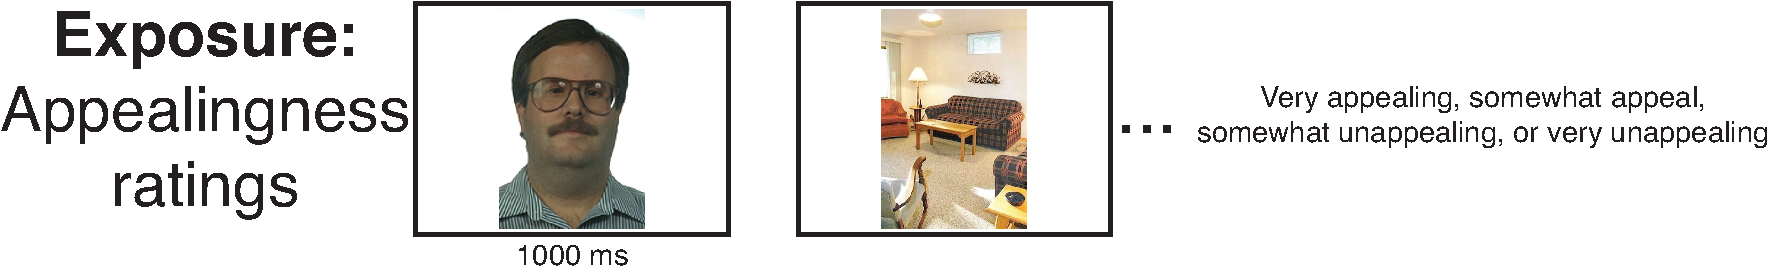
\includegraphics[width=.8\textwidth]{./figs/exp1/space_example_expo} \\
%   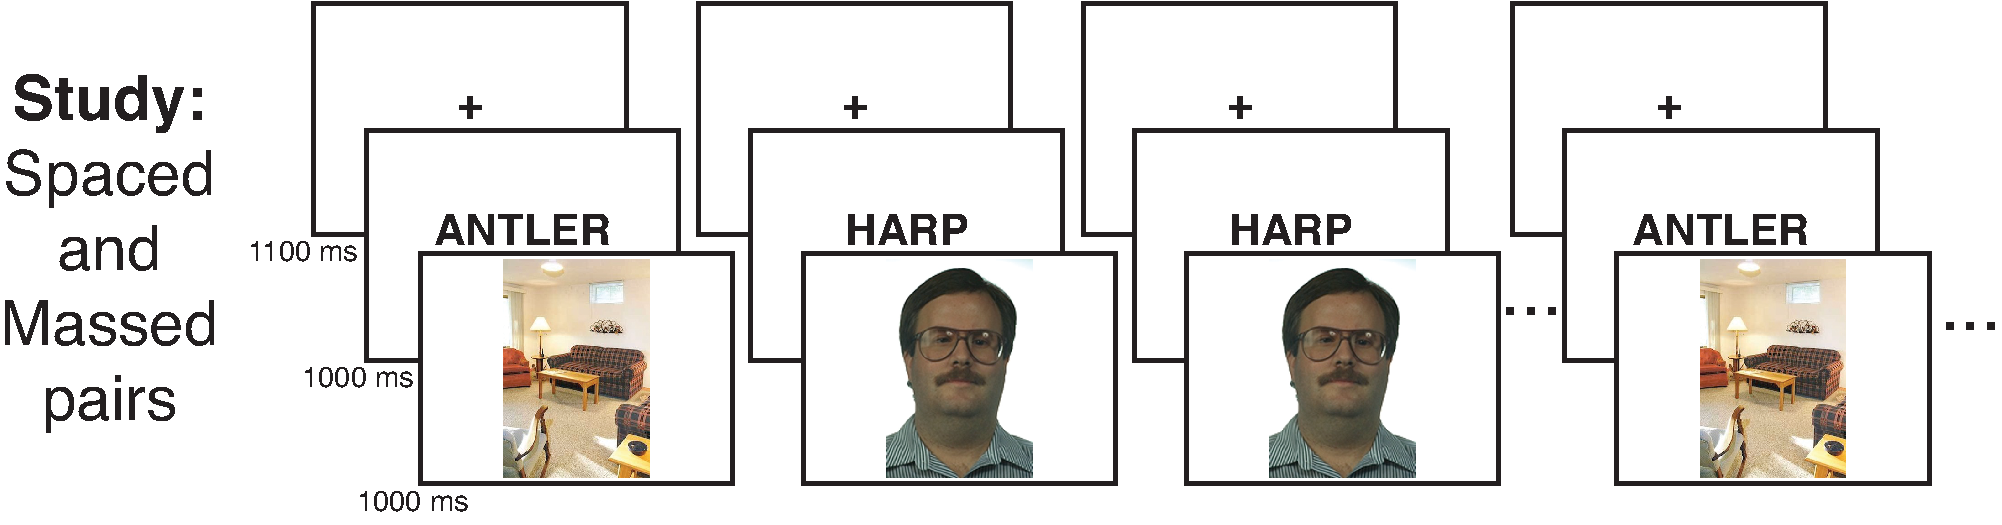
\includegraphics[width=.9\textwidth]{./figs/exp1/space_example_study_fix} \\
%   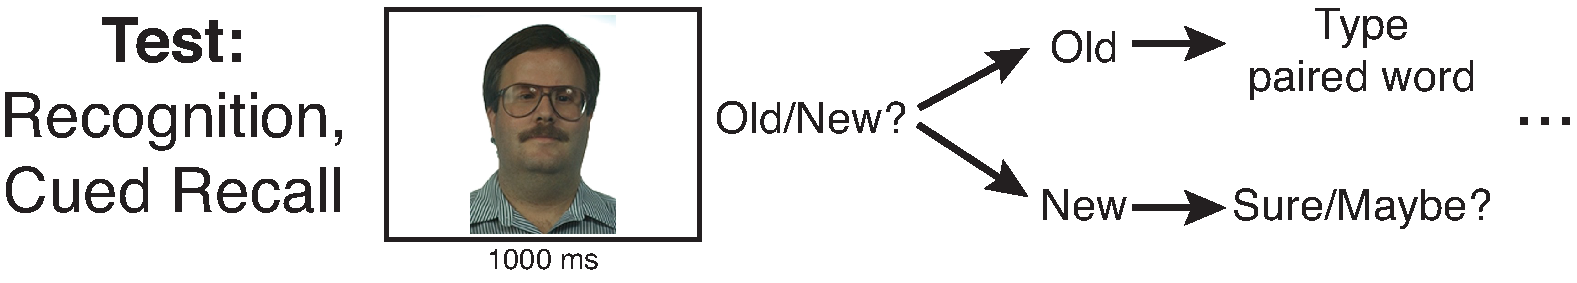
\includegraphics[width=.7\textwidth]{./figs/exp1/space_example_test}
%   \end{tabular}
%   \caption{Experiment~1: Exposure, study, and test phases}
%   \label{fig:space2_exp}
%   %\label{fig:space2_study}
%   %\ref{fig:space2_study}
%   %\pageref{fig:space2_study}
% \end{figure}

% for each category, 3 image trials of each of 5 types: 

% (((9+3)*2)+3+2)*2

In each study phase block, participants viewed word--image pairs and were asked to think of a relationship between them or to make up a story pairing them.  They were told that a subsequent test would require them to remember the word associated with each picture, but they were not told that some pairs are repeated.  Spaced items were presented at a lag of either 2, 12, or 32, and massed items were presented at a lag of zero.  For each of the two image categories there were three two-presentation spaced pairs per lag, three two-presentation massed pairs, three pairs presented only once, and four additional single-presentation buffers (two at the beginning of the list and two at the end).
% All images (including spaced, massed, and single presentation items) were included on the test list.
Thus, there were 58 word--image presentations in each block.  On each trial, a fixation cross appeared for 1.0--1.2~s (jittered), then the word was presented first for 1.0~s followed immediately by the image for 1.0~s.  No more than three images from the same category could occur in a row, and no more than two trials with the same lag (including single-presentation pairs) could occur in a row.  Each study phase lasted approximately \hl{5~min}.

In the distractor phase, participants answered simple math problems of the format \texttt{A+B+C=?} for 2~min.  They typed their responses with the keyboard.  Different tones occurred for correct and incorrect answers, and mean accuracy and response time was reported to the participant at the end of the phase.

% \begin{figure}
%   \centering
%   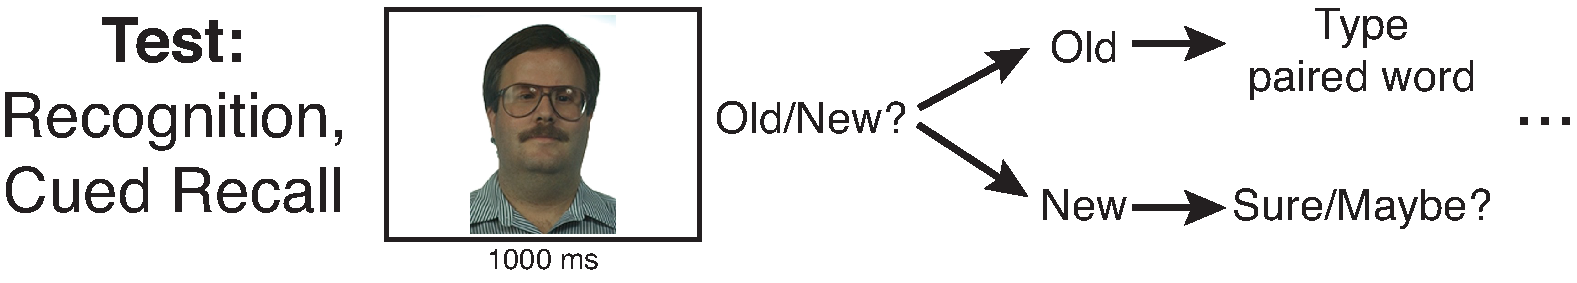
\includegraphics[width=\textwidth]{./figs/exp1/space_example_test}
%   \caption{Experiment~1: Test phase}
%   \label{fig:space_test}
%   %\ref{fig:space_test}
%   %\pageref{fig:space_test}
% \end{figure}

Finally, in the test phase, participants performed a cued recall task.  Thirty images (nine spaced, three massed, and three single presentation images from each category) were mixed together and presented one at a time.  Participants saw \texttt{???????} below each image and had to type the word previously paired with the image; they could pass if they could not remember the word.  On each trial, a fixation cross appeared for 1.0--1.2~s (jittered) and the image was shown for 1.0~s, at which point the question marks appeared and participants were asked to make their response.  Importantly, test images were presented in a sequence similar to the study order.  To construct the test list, the positions of the second presentations of study stimuli were divided into fifteen contiguous groups and each group was shuffled internally.  This was done to approximately preserve a similar amount of time between the second presentation and the test across all ``old'' stimuli.  Each test phase lasted approximately \hl{4 to 5~min}.

% 3.0~s timer for recognition and new responses

% There were approximately 7~min between studying a spaced or massed word--image pair and seeing that image on the test list.

\subsubsection{Electrophysiological recordings and data processing}

The procedure for recording and processing electrophysiological data was the same as in Experiment~1.

The same methodology was used to find peak electrodes and latencies for analyzing ERP effects.  Peaks in Experiment~2 were at the same electrodes as in the previous experiment, but were slightly earlier in time.
The visual N1 peaked at electrode~58 (T5) peaked at $144$~ms (Figure~\ref{fig:s2_N1}; $\pm$50~ms window).  The N400 peaked at Cz at $352$~ms (Figure~\ref{fig:s2_N400}; $\pm$50~ms window).  The LPC peaked at electrode~77 at $536$~ms (Figure~\ref{fig:s2_LPC}; $\pm$100~ms window).  Again, analyses use these peak electrodes and neighbors during study period words stimuli.

Time--frequency processing and analyses also followed the same procedures as in Experiment~1.

\subsection{Results}

% DNF session 2:
% SPACE2003
% SPACE2009
% SPACE2013 % didn't record EEG so stopped in middle of session 1
% SPACE2020
% SPACE2023
% SPACE2024
% SPACE2027
% SPACE2039

% performance more than 2 STD below mean in some cases (e.g., lag 32):
% SPACE2007 (also rejected below)
% SPACE2025 (also rejected below)

% EEG trials < 10:
% SPACE2002 (also rejected below)
% SPACE2007 (also rejected above)
% SPACE2025 (also rejected above)
% SPACE2034

% noisy EEG:
% noisiest first: 2, 16, 22, 40, 26, 36, 10, 17; only rejecting 2 and 16
% SPACE2002 (also rejected above)
% SPACE2016

Ten participants were excluded from all analyses either because they did not return for the required second session ($n=8$) or their performance in important conditions was more than 2 standard deviations below the mean ($n=2$).  The remaining thirty participants were included in behavioral analyses.

Three additional participants were excluded from ERP and time--frequency analyses either because they had extremely noisy EEG ($n=2$) or had fewer than 10 artifact-free trials in any of the main trial conditions ($n=1$), leaving twenty-seven participants in EEG analyses.  Similarity analyses included the \hl{??} participants who had six or more artifact-free pairs of initial presentation--repetition image trials; images were used because this is when word--image (item--context) binding should occur.

All analyses contingent on subsequent memory are split by whether words were recalled or forgotten after the image was correctly recognized as being old.

\subsubsection{Behavioral results}

An ANOVA with factors of session (1 and 2), spacing (single presentation, massed, short, medium, and long spaced), and image category, was run on cued recall hit rate.  There was a main effect of spacing [$F(1,29)=174.2, p=0$] in the expected order: long spaced words ($M=56.9\%$) were recalled better than medium spaced words ($M=49.2\%$), and in turn performance for each of short spaced ($M=45.8\%$), massed ($M=35.7\%$), and single presentation words ($M=23.0\%$) was better than the next.  Words paired with faces and scenes were recalled at the same rate (faces: $M=44.0\%$; scenes: $M=40.2\%$).  Thus, there are again clear spacing effects that scale with spacing, as well as a simple repetition effect. These rates are comparable to Experiment~1.

There were also session $\times$ image category [$F(1,29)=7.96, p=.0086$] and spacing $\times$ image category [$F(4,116)=7.52, p=4.47e^{-05}$] interactions such that recall was better for faces in session 1 compared to session 2, and performance increased at the longest lag for faces compared to scenes.  However, these effects do not speak to our investigations of the spacing effect and will not be reported in detail.

\subsubsection{ERP results}

Again, during studied words the visual N1 peaked at 144~ms (Figure~\ref{fig:N1}), the N400 peaked at 352~ms (Figure~\ref{fig:N400}), and the LPC peaked at 536~ms (Figure~\ref{fig:LPC}).  Significant results are reported.

\subsubsection{ERP discussion}



\subsubsection{Time--frequency results}



\subsubsection{Time--frequency discussion}



\subsubsection{Similarity results}



\subsubsection{Similarity discussion}



\subsection{Experiment~1 Discussion}


